\section{Data Preprocessing}
% ─────────────────────────────────────────────────────────────

To construct the final structured input for both classical and deep learning models, we developed an offline preprocessing pipeline. This pipeline enforces mathematical consistency and strict separation between evaluation folds. The processing sequence is structured as follows:

\begin{enumerate}
    \item \textbf{Data Cleaning:} Column names were stripped of leading/trailing whitespaces to avoid structural reference errors. We identified invalid numerical entries, including missing values (\texttt{NaN}) and infinite calculations (\texttt{inf}) arising from division-by-zero errors in flow rate features (e.g., \texttt{Flow Bytes/s}). These rows constituted less than 0.1\% of the raw data and were dropped directly, avoiding synthetic imputation bias.
    \item \textbf{Dimensionality Reduction:} Statistical profiling of the 78 raw features identified columns with zero variance (e.g., constant TCP flags or empty bulk rate columns) and non-numeric metadata columns. Programmatically removing these constant and non-numeric features reduced our input dimensionality from 78 to 70 active features, mitigating computational complexity and reducing collinear noise. The redundant correlation structure of the highest-variance features is visualized in Figure~\ref{fig:feature_corr}.
    \item \textbf{Stratified Sampling:} Given that the full CIC-IDS2017 dataset exceeds 2.8 million rows, training distance and kernel-based models with quadratic complexity ($\mathcal{O}(n^2)$) is computationally prohibitive. A 20\% stratified random sample was extracted, yielding approximately 565,000 instances while precisely preserving the native class ratio of 80.3\% benign and 19.7\% anomalous traffic.
    \item \textbf{Stratified Split and Scaling:} The stratified sample was partitioned into 70\% Training, 15\% Validation, and 15\% Testing sets. To ensure proper convergence of distance-based models (LOF, OC-SVM) and neural networks (Autoencoders), features were normalized using \textit{StandardScaler}. To prevent data leakage, the scaler was fitted exclusively on the Training partition and subsequently applied to transform the Validation and Test sets.
\end{enumerate}

\begin{figure}[H]
    \centering
    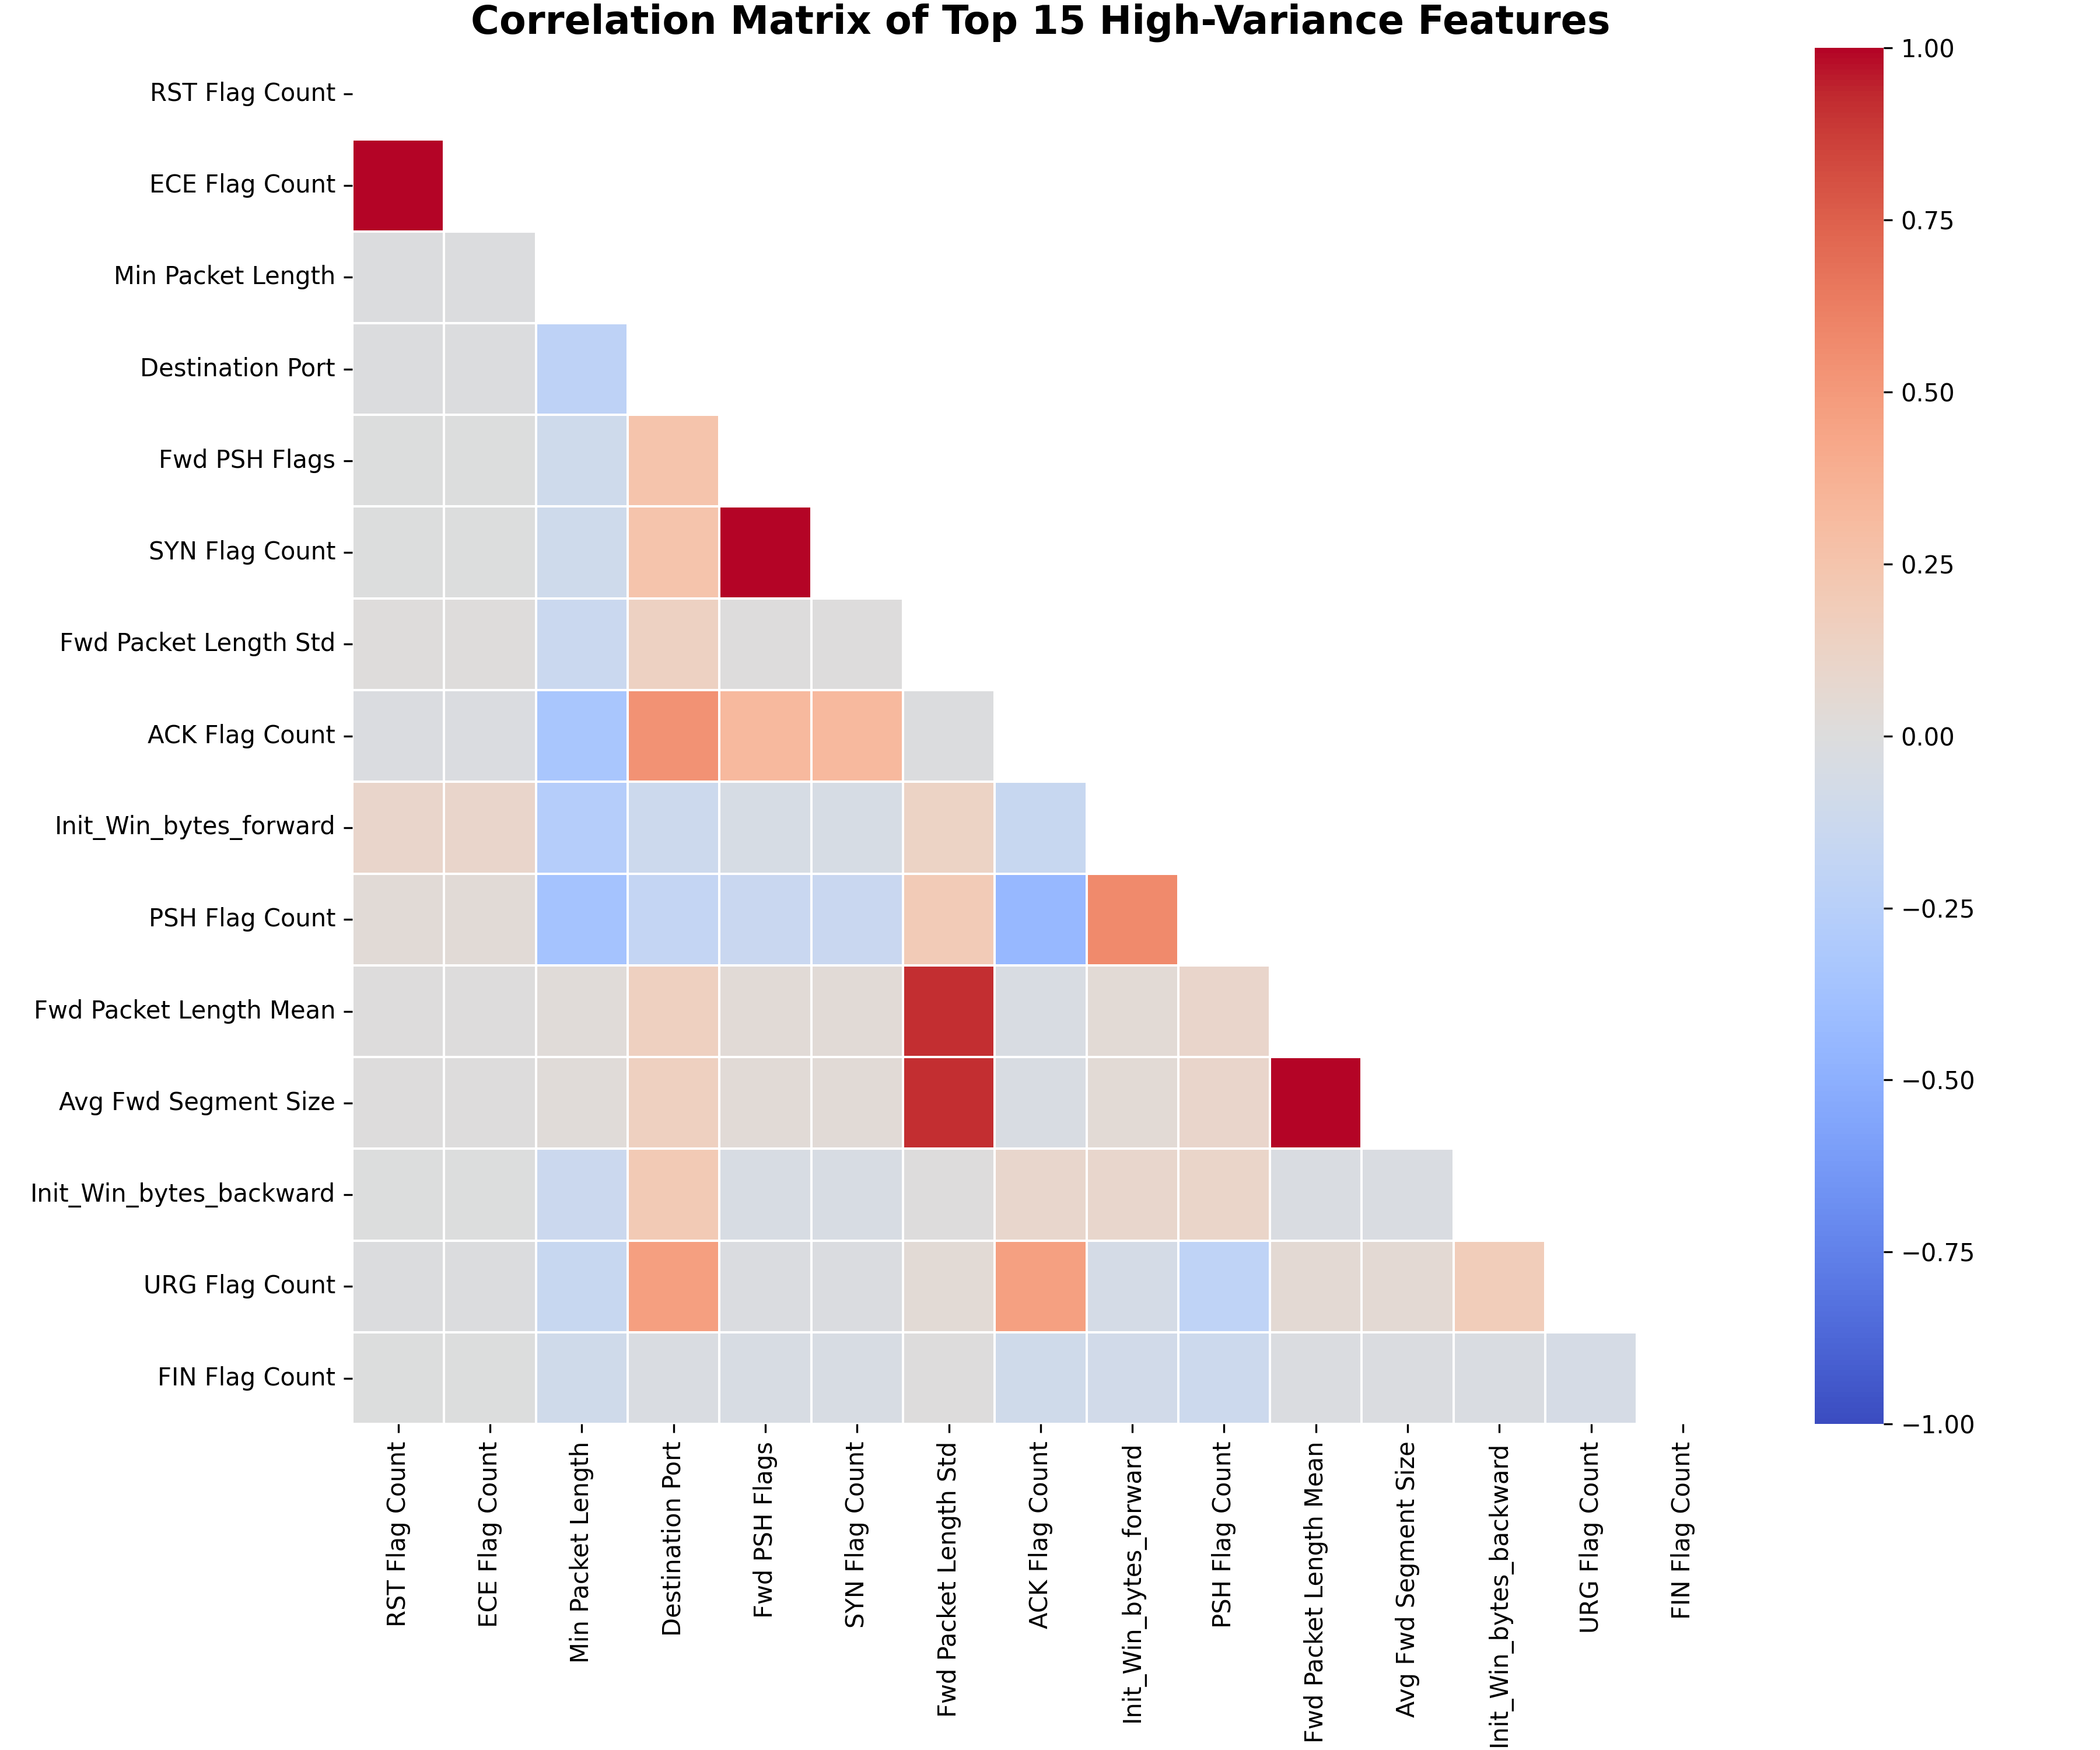
\includegraphics[width=0.95\columnwidth]{images/feature_correlation.png}
    \caption{Correlation matrix heatmap of the top 15 high-variance features post-preprocessing. The high density of near-perfect correlations ($r \approx 1.0$) illustrates the significant feature redundancy inherent in raw flow statistical captures, justifying feature pruning.}
    \label{fig:feature_corr}
\end{figure}
